\chapter{In-Flight Procedures}

% This is true if only doing the flight manual, not the pre-flight
\ifisflight
  % This one page needs to be one column to look right, even
  % in the flight manual, proper.
  % failed experiment to add thumb guides
%   \addthumb{Welcome}{}{white}{black}
\putchapterthumb
\fi


Once you're at \gls{ttm}, you'll want to keep gate hours in mind (if you leave), and before you finally pack up to go to your rest-of-the-year home, please take a moment to read through our takeoff procedure!

\section*{Gate Hours}

\textbf{No vehicles will be allowed in after sunset! No moving vehicles \textit{period} inside the burn when it's dark - so if you get there right before sunset, you better get in, unload your stuff, and get right back out to parking ASAP. This is for the safety of everyone at the burn!}

Any vehicles that arrive after sunset will be redirected to parking, where we may or may not have a golf cart to help you carry some stuff in --- but don't count on it --- use that Radical Self-Reliance!

\begin{table*}[h!]
\footnotesize
\centering
\caption{\Gls{ttm} \gls{gate} hours}
\label{tbl:gatehours}
\begin{tabular}{@{}lll@{}}
\toprule
Wednesday & 6/12/2019 & 12--10\pm EST                                    \\ 
          &           & Theme Camp Early Entry Only w/ Pre-Registration \\
Thursday  & 6/13/2019 & 10\am--12\am EST                                   \\
Friday    & 6/14/2019 & 10\am--12\am EST                                    \\
Saturday  & 6/15/2019 & 10\am--6\pm EST, no admission after 6pm for rest of event \\
Sunday    & 6/16/2019 & 10\am--6\pm EST                                    \\
          &           & Departing Only                                  \\
Monday    & 6/17/2019 & 8\am--12\pm EST                                    \\
          &           & Departing Only                                  \\ \bottomrule
\end{tabular}
\end{table*}

\section*{Re-entry Procedure}

\textbf{There is no after hours entry without pre-arranged permission.  Crew arriving at the site outside gate operating hours will be turned away.  No crew is permitted to wait on the property until the gate opens.}

Please contact the \gls{bod} via \url{connect@tothemooonburn.com} well in advance of the event to work out options if long-distance travelers cannot arrive while the gate is open.

For the safety of other patrons and to preserve the integrity of the experience, \textbf{no} coming and going at leisure is allowed after checking in.  Exiting and returning \gls{ttm} are reserved \textbf{for medical and emergency reasons only}, and must be communicated to and cleared by the Gate Lead prior to leaving.

Theme Camp supply runs are possible Wednesday -- Friday before 10\pm \textbf{only}. Before leaving, \textbf{check at the gate} if a pass is needed. The Gate will check with \Gls{el} on call and a re-entry lanyard will be issued at \gls{el} discretion.

% If you forget something and need to ``make a run to the store'' talk to a team / event  / gate lead and we can grant Re-Entry if you combine your trip with one beneficial \gls{ttm} and the community at large.

\section*{Takeoff Procedure}
\subsection*{Leave No Trace}
\Gls{ttm} follows the \gls{lnt} principle (see \gls{tenprinciples}, page \pageref{tenprinciples}). Please take all your belongings, trash, and \gls{graywater} with you and leave the site in a better shape than you found it.

\subsection*{Takeoff Launch Window}

\Gls{ttm} officially closes at 11:59\pm EST, Sunday, June 17th.  All crew must vacate the site by 12pm EST, Monday, June 18th unless given explicit prior permission from Theme Camp Late Departure.

Vehicles can be driven on site on Monday to pack up. In case of inclement weather, a no driving / limited access policy to site will be implemented. Be prepared by bringing your own cart / wagon to transport gear out and to your vehicle.
\Gls{love} will be able to assist with shuttling gear to parking. 
Vehicles can \textbf{not} be parked alongside road to do so, but only be lined up at gate about 10 at a time.

Pleases look for announcements at \Gls{cockpit} / \Gls{gate}, as this policy may slightly change, depending on situation. 

\newpage
\section*{Resources}

% \begin{wrapfigure}{R}{0.3\textwidth}[h!]
% \centering
% 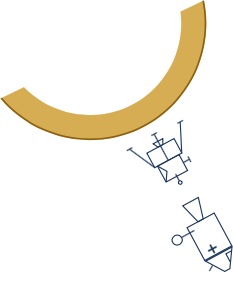
\includegraphics[width=0.25\textwidth]{images/landing1.png}
% % \caption{}
% \end{wrapfigure}
% \begin{multicols}{2}
\subsection*{Showers}
There are no showers. To keep yourself clean, bring wet wipes or biodegradable soap.
Please don't clean your dishes or yourself in the river since there are mussels in the river that are protected wildlife.  (And these are also the reason you should wear river shoes while in the river as the mussels will cut you. They're mean that way.)

\subsection*{Ice}
Ice will be soled from noon to 3 \pm every day for \$2 per 10 lbs bag.  Cash only! Bring small bills please. 


\subsection*{Lost and Found}
The Lost and Found will be at the \gls{cockpit} / \gls{vc} station.

\subsection*{Port-a-Potties}
There are Port-a-Potties on-site. Please don't put anything other than one-ply toilet paper and human waste in the Port-a-Potties. You will find Port-a-Potties in multiple locations across the site.



% \reflectbox{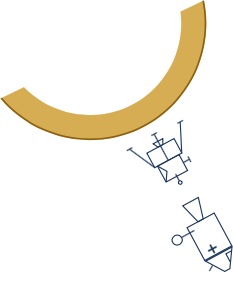
\includegraphics[width=\columnwidth,angle=180]{images/landing1.png}}

% \vspace*{\fill}
\ifisflight
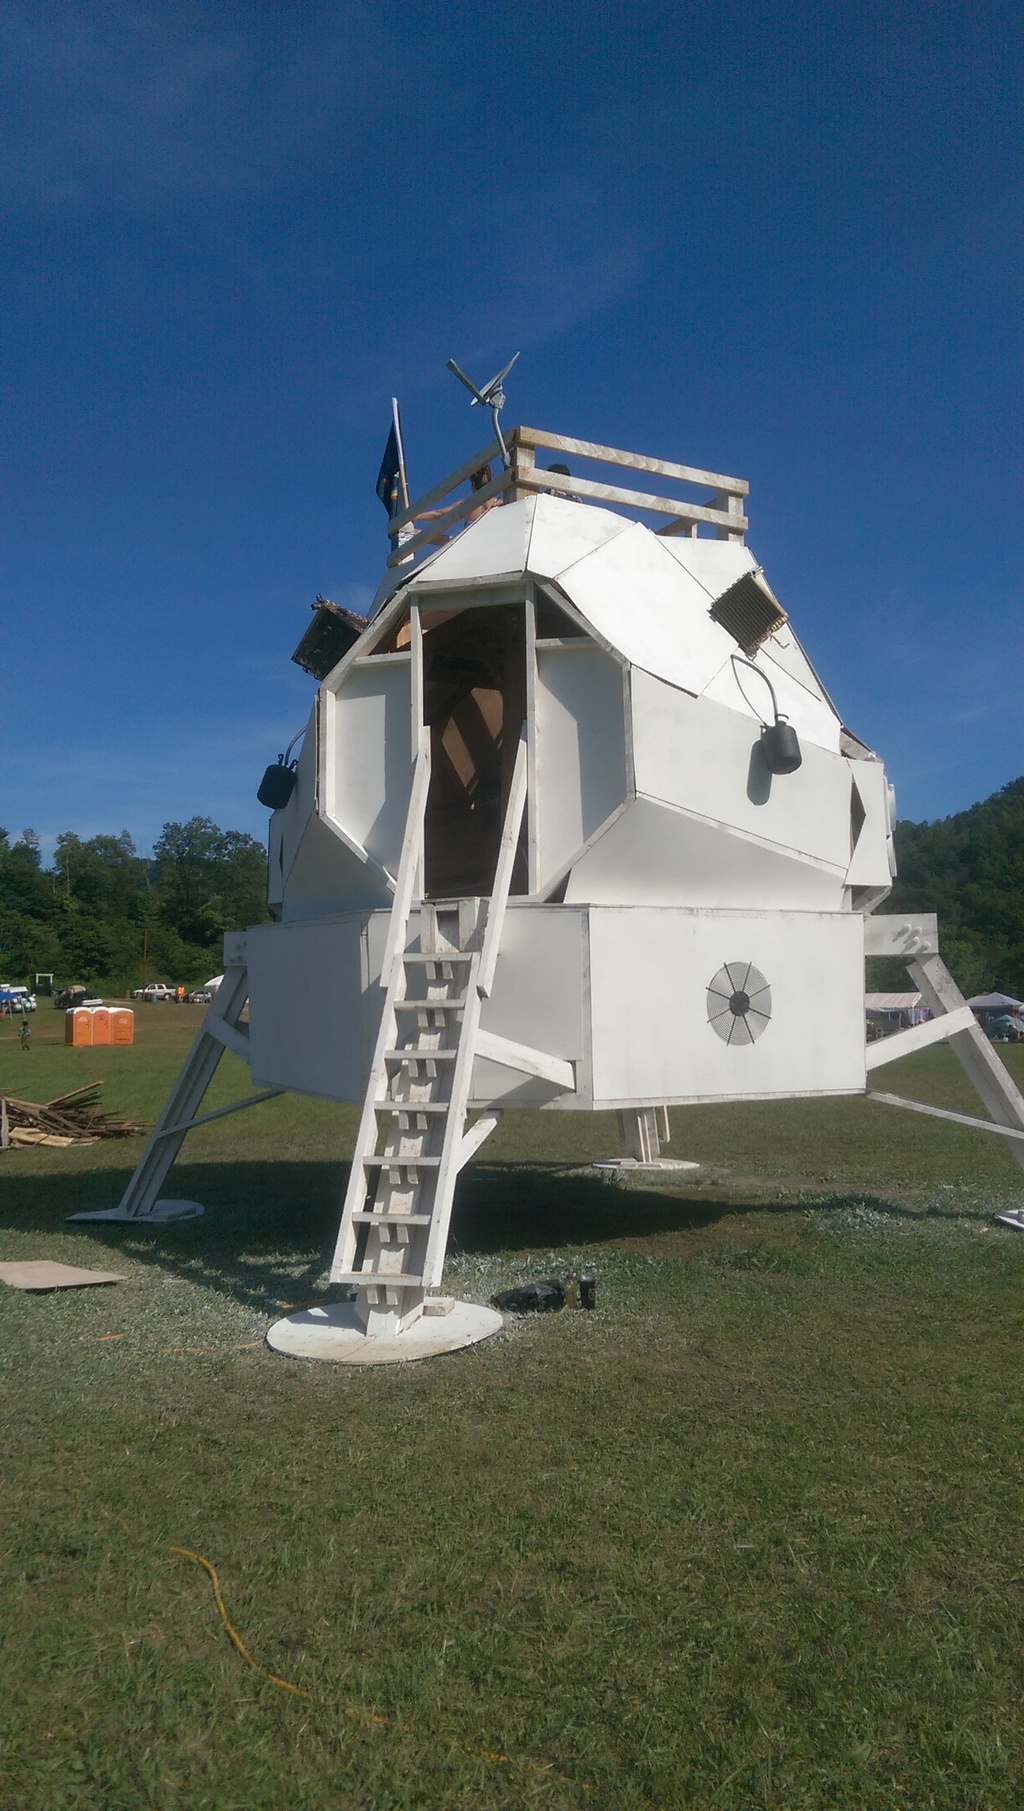
\includegraphics[width=\columnwidth]{images/2017Effigy_small.jpg}
\fi